\section{SCGRA Overlay Infrastructure} \label{sec:scgraimplement}
One key idea of QuickDough is to rely on an intermediate SCGRA overlay to improve compilation time of the high-level user application. While the exact design of this SCGRA does not affect the compilation flow, its implementation does have a significant impact on the performance of the generated gateware.
 
\subsection{SCGRA Based FPGA Accelerator}
\figref{fig:scgra-accelerator} presents the proposed FPGA accelerator built on top of an SCGRA overlay. The input/output data buffers and Acc-Ctrl block are the same with those in the typical acceleration architecture in \figref{fig:typical-FPGA-accelerator}, while the computation core is unique. It consists of an array of synchronous PEs which can be easily pipelined and run at higher frequency. Moreover, the regular array is able to maintain the high implementation frequency even when it scales up.

On top of the computation core, the accelerator has two address buffers (Addr IBuf/OBuf) instead of customized logic to control the on-chip data buffer accessing. When target application changes, the user can simply update the content of the address buffers to adapt to the change and thus can reuse the same hardware structure, which is beneficial to design reuse and improving design productivity. 

Another important block of the accelerator is SCGRA-Ctrl. It can be used to iterate the SCGRA execution until the executions consume all the data in input data buffer or fill the output data buffer. As the executions can share the same input/output data buffer, it helps to increase the data reuse and reduce the communication cost. 

\begin{figure}[h]
    \center{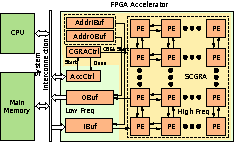
\includegraphics[width=0.8\linewidth]{scgra-accelerator}}
    \caption{SCGRA Overlay Based FPGA Accelerator}
    \label{fig:scgra-accelerator}
\end{figure}

\subsection{Processing Element (PE)}
In this section, an instance of the pipelined PE is presented to demonstrate the feasibility of producing high performance gateware. As shown in \figref{fig:pe}, the PE, centring an ALU block, a multiple-port data memory and an instruction memory, is highly optimized for FPGA implementation. In addition, load/store paths are implemented on the PEs that are responsible for data I/O beyond the FPGA. Addr-Ctrl is used to start and reset the SCGRA execution by changing the instruction memory read address. In order to synchronize the execution of the PE array, each PE has a single bit global start signal from the SCGRA-Ctrl block. 

\begin{figure}[h]
\center{\includegraphics[width=0.95\linewidth]{pe}}
\caption{Fully Pipelined PE structure}
\label{fig:pe}
\end{figure}

\subsubsection{Instruction Memory and Data Memory}
The instruction memory stores all the control words of the PE. Its content will not change at runtime, so ROM is used to implement this instruction memory. The address of the instruction ROM is determined by the Addr-Ctrl. Once the start signal is valid, the ROM address will increase by one every cycle and the SCGRA execution will proceed accrodingly. When the start signal is invalid, the ROM address will be reset to be 0 and the SCGRA execution will stop.

Data memory stores intermediate data that can either be forwarded to the PE downstream or be sent to the ALU for calculation. For fully parallelized operation, at least \emph{four} read ports are needed -- three for the ALU and one for data forwarding. Similarly, at least two write ports are needed to store input data from upstream memory and to store the result of the ALU in the same cycle. Although a pair of true dual port memories seem to meet this port requirement, conflicts may arise if the ALU needs to read the data while the data path needs to be written. As a result, a third dual port memory is added to the data memory.

\subsubsection{ALU}
At the heart of the proposed PE is an ALU designed to cover the computations in the target applications. \figref{fig:ALU} shows an example design that can support all the operations of our benchmark as listed in \tabref{tab:operations}. As the operations are usually different, each operation is provided with an independent data path. At the end of the data paths, a set of multiplexers are added to select the expected output. Currently, the maximum number of operations allowed in this template is 16 and an additional pipeline stage is added for the output selection. As the scheduler will make sure that the output port of the ALU is contention-free, the opcode in this ALU doesn't have to align with the input operations. Instead, it is merely used for output selection. Therefore, the proposed ALU can be easily customized and scaled.

\begin{figure}[h]
\center{\includegraphics[width=0.8\linewidth]{alu-v2}}
\caption{ALU Example Supporting 12 Operations}
\label{fig:ALU}
\end{figure} 

\begin{table}[h]
\caption{Operation Set Implemented in ALU}
\label{tab:operations}
\centering
\begin{tabular}{l|c|l}
\hline
Type & Opcode & Expression \\

\hline
MULADD & 0001 & {dst = (src0 $\times$ src1) + src2} \\

\hline
MULSUB & 0010 & {dst = (src0 $\times$ src1) - src2} \\

\hline
ADDADD & 0011 & {dst = (src0 + src1) + src2} \\

\hline
ADDSUB & 0100 & {dst = (src0 + src1) - src2} \\

\hline
SUBSUB & 0101 & {dst = (src0 - src1) - src2} \\

\hline 
PHI & 0110 & {dst = src0 ? src1 : src2} \\

\hline
RSFAND & 0111 & {dst = (src0 $\gg$ src1) \& src2} \\

\hline
LSFADD & 1000 & {dst = (src0 $\ll$ src1) + src2} \\

\hline
ABS & 1001 & {dst = abs(src0)} \\

\hline
GT & 1010 & {dst = (src0 $>$ src1) ? 1 : 0} \\

\hline
LET & 1011 & {dst = (src0 $\leq$ src1) ? 1 : 0} \\

\hline
ANDAND & 1100 & {dst = (src0 \& src1) \& src2} \\

\hline
\end{tabular}
\end{table}

\subsection{Load/Store Interface}
For the PEs that also serve as IO interface to the SCGRA, they have additional load path and store path as shown in \ref{fig:pe}. Load path and the SCGRA neighboring input share a single data memory write port, and an additional pipeline stage is added to keep the balance of the pipeline. Store path has an additional data multiplier as well, but it doesn't influence the pipeline of the design. 

